\documentclass[11pt]{beamer}


\usepackage{amssymb, amsmath, graphicx, caption, enumerate}
\graphicspath{ {images/} }
\usepackage{amsthm}
\usepackage{xargs}
\usepackage{scalerel}




\newcommand{\N}{\mathbb{N}}
\newcommand{\Z}{\mathbb{Z}}
\newcommand{\R}{\mathbb{R}}
\newcommand{\K}{\mathbb{K}}
\newcommand{\C}{\mathbb{C}}
\newcommand{\D}{\mathcal{D}}
\newcommand{\A}{\mathcal{A}}
\newcommand{\ds}{\displaystyle}
\newcommand{\op}[1]{\left(#1\right)}
\newcommand{\cp}[1]{\left[#1\right]}
\newcommand{\av}[1]{\left| #1\right|}
\newcommand{\st}[1]{\left\{#1\right\}}


\usepackage[colorinlistoftodos,prependcaption,textsize=tiny]{todonotes}
\newcommandx{\question}[2][1=]{\todo[linecolor=red,backgroundcolor=red!25,bordercolor=red,#1]{#2}}
\newcommandx{\change}[2][1=]{\todo[linecolor=blue,backgroundcolor=blue!25,bordercolor=blue,#1]{#2}}
\newcommandx{\add}[2][1=]{\todo[linecolor=OliveGreen,backgroundcolor=OliveGreen!25,bordercolor=OliveGreen,#1]{#2}}
\newcommandx{\improve}[2][1=]{\todo[linecolor=Plum,backgroundcolor=Plum!25,bordercolor=Plum,#1]{#2}}
\newcommandx{\thiswillnotshow}[2][1=]{\todo[disable,#1]{#2}}
\newcommandx{\remove}[2][1=]{\todo[linecolor=yelllow,backgroundcolor=yellow!10,bordercolor=red,#1]{#2}}


\newcommand\reallywidehat[1]{\arraycolsep=0pt\relax%
\begin{array}{c}
\stretchto{
  \scaleto{
    \scalerel*[\widthof{\ensuremath{#1}}]{\kern-.5pt\bigwedge\kern-.5pt}
    {\rule[-\textheight/2]{1ex}{\textheight}} %WIDTH-LIMITED BIG WEDGE
  }{\textheight} % 
}{0.5ex}\\           % THIS SQUEEZES THE WEDGE TO 0.5ex HEIGHT
#1\\                 % THIS STACKS THE WEDGE ATOP THE ARGUMENT
\rule{-1ex}{0ex}
\end{array}
}


\usetheme{CUDenver}
\renewcommand{\familydefault}{\sfdefault}
\usefonttheme[onlymath]{serif}
\usepackage{tikz}
\usetikzlibrary{arrows}
\setbeamertemplate{itemize items}{>>}
\setbeamertemplate{itemize subitem}[square]
\setbeamertemplate{itemize subsubitem}[ball]
\newcommand{\norm}[1]{\left\lVert#1\right\rVert}



\author{Jordan R. Hall}

\title[CUDenver Theme]{Optimizing Noisy Functions with Machine Learning}

\institute[UCD]{
Department of Mathematical and Statistical Sciences\\
University of Colorado Denver
}

\date{Friday, February 1, 2019}

\begin{document}
% ------------------------------------------------


\begin{frame}[t,plain]
    \titlepage
\end{frame}

% start the content of the presentation

\begin{frame}{Overview}

\tiny
\tableofcontents
\end{frame}


% ------------------------------------------------
\section{Introduction}
% ------------------------------------------------

\begin{frame}

\begin{block}{Notation}



\begin{itemize}

	\item We define a model parameter space $\Lambda$ with dimension $N$ and a data space $\mathcal{D}$ with dimension $M$. 
	\begin{itemize}
		\item In most settings, $\Lambda$ will be of higher dimension than $\mathcal{D}$.
	\end{itemize}
	
	\item We define a parameter-to-data map $f:\Lambda\rightarrow \mathcal{D}$, 
	\begin{itemize} 
	 	\item $f$ may be polluted by noise.
		\item  $\nabla f$ may be inaccessible.	
	\end{itemize}
	
	\item We write $d=f(\lambda) \in \mathcal{D}$ to denote a particular datum corresponding to the evaluation of a point $\lambda \in \Lambda$. %\alphax
	
	%\item We note a probability distribution function of a random variable x as

\end{itemize}

\end{block}

\end{frame}



% ------------------------------------------------
\subsection{Dimension Reduction}
% ------------------------------------------------

\begin{frame}

\begin{itemize}

	\item We consider functions $f: \Lambda \to \mathcal{D}$ where $\dim(\Lambda)=N$ is large and $\dim(\mathcal{D})=M$ is such that $M<N$ or $M<<N$.

\begin{itemize}
		\item Functions of interest may represent postprocessed quantities from the solution of complex physical models.
\end{itemize}

\item It is not often that every parameter has equal impact on function values -- usually some parameters matter more than others.

\item The dimension reduction techniques considered seek to explain outputs $f(\Lambda)$ in an \textit{active subspace} $\mathcal{A} \subset \Lambda$ for which $\dim(\A)<N.$

\begin{itemize}
\item Many common uses (e.g., statistics) of $f$ involve integration over $\Lambda$ and are subject to the \textit{curse of dimensionality}.
\item This forces the use of Monte Carlo or Quasi-Monte Carlo methods.
\item A lower-dimensional representation of $f$ may enable faster methods.
\end{itemize}


\end{itemize}


\end{frame}

\begin{frame}

\begin{itemize}

\item $\nabla f(\lambda)\in \Lambda$ is a column vector containing the $N$ partial derivatives of $f$, which for this discussion we assume exist, and are square integrable in $\Lambda$ equipped with some probability density that is positive everywhere in $\Lambda$ and 0 otherwise.

\begin{itemize}
		\item We consider $\pi_\Lambda^\text{prior}(\lambda)$, the density describing our prior state of knowledge, which we abbreviate as $\pi_\Lambda$.
\end{itemize}

\item For convenience, one transforms inputs $\lambda$ to the origin with some fixed variance, typically so that $\lambda\in [-1,1]^N$. We define

\end{itemize}

\begin{block}{Covariance in Gradient Space \footnotemark[1]}

\begin{equation} \label{eq:4}
W=\int_\Lambda \nabla f(\lambda) \nabla f(\lambda)^\top  \pi_\Lambda(\lambda) d\lambda,
\end{equation} 

\noindent which is an $N\times N$ symmetric positive semi-definite matrix.

\end{block}

%\footnotetext[1]{Constantine, Eftekkari, Wakin}
\footnotetext[1]{Constantine, \textit{Active Subspaces: Emerging Ideas for Dimension Reduction in Parameter Studies}}


\end{frame}

\begin{frame}

\begin{itemize}



\item Interpreting $W$ as a certain covariance structure over $\Lambda$ leads one to the idea of computing the Singular Value Decomposition of $W$,

\begin{block}{Singular Value Decomposition (SVD) of $W$}

\begin{equation} \label{eq:5}
W=U\Sigma V^*,
\end{equation} 


\noindent where $U$ is $N \times N$ unitary, $\Sigma$ is $N \times N$ diagonal with the singular values of $W$ along its diagonal, and $V^*$ is $N \times N$ unitary.

\end{block}

\item We plot the singular values, $\{\sigma_i\}_{i=1}^n$ and seek a drop-off in magnitude between some pair of singular values, $\sigma_{j}$ and $\sigma_{j+1}$. The active subspace is the span of $u_1,\ldots,u_{j}$, which are the first $j$ columns of $U$, the left singular vectors of $W$. 


\end{itemize}

\end{frame}

\begin{frame}

\begin{itemize}

	\item For a point $\lambda \in \Lambda$, we define

\begin{block}{Projection into $\mathcal{A}$, \textit{active variables}}

\begin{equation} \label{eq:6}
  \mathcal{P}_\A(\lambda)=\sum_{i=1}^{j}\left( u_i^T \lambda\right)u_i, 
\end{equation}

\noindent which is the projection of $\lambda$ in the active directions of $f$.

\end{block}

\item We have arrived at the property that 

\begin{block}{Resolution of $f$ in $\mathcal{A}$}

\begin{equation} \label{eq:7}
f\left(\mathcal{P}_\A(\lambda)\right) \approx f(\lambda).
\end{equation}

\end{block}

\end{itemize}



\end{frame}


\begin{frame}

\begin{itemize}

\item Finding an active subspace requires forming an approximation to $W$ via Monte Carlo. Here we consider techniques in \footnotemark[1] \footnotemark[2].



\item We let $D_S=\{(\lambda_i,f(\lambda_i))\}_{i=1}^S$, which is a set of $S$ pairs of samples $\lambda_i \in \Lambda$ and their function values. 

\item One may use $D_S$ to approximate $\nabla f$. We denote each estimation to $\nabla f(\lambda_i) \approx \reallywidehat{\nabla f}(\lambda_i)$.

\item We form the $N \times S$ matrix $\tilde{W}$ (which we present as $\tilde{W}^\top$)

\end{itemize}

\begin{block}{Monte Carlo Approximation to $W$ \footnotemark[1]}


\begin{equation} \label{eq:4}
\tilde{W}^\top:=\begin{bmatrix}
\reallywidehat{\nabla f}(\lambda_1)
\cdot \cdot \cdot
\reallywidehat{\nabla f}(\lambda_S)\\
\end{bmatrix}.
\end{equation}  

\end{block}

\footnotetext[1]{Russi, \textit{UQ with Experimental Data and Complex System Models}}
\footnotetext[2]{Constantine et al, \textit{Computing Active Subspaces Efficiently with Gradient Sketching}}

\end{frame}


\begin{frame}

\begin{itemize}

	\item Forming the SVD of $\tilde{W}$, $\tilde{W}=\tilde{U}\tilde{\Sigma}\tilde{V}^*$, we search for a drop off in the magnitude of the singular values $\{\tilde{\sigma}_i\}_{i=1}^S$. Assuming such a drop off occurs for an index $j:1<j<S$, we have the $j$ corresponding left singular vectors,$ \tilde{u}_1,\ldots,\tilde{u}_{j}$.  
	
	\item Then we define

	\begin{block}{Monte Carlo approximation to $\A$}
	
	
	$$\A\left(f; D_S \right):=\text{span}\{\tilde{u}_1,\ldots,\tilde{u}_{j}\},$$ the active subspace of $f$ with respect to the samples $D_S$.
	
	\end{block}		

	\item For low dimensional $\A$, we may check $f(\mathcal{P}_\A(\lambda))\approx f(\lambda)$ in a \emph{sufficient summary plot}, where we plot active variables against function values.


\end{itemize}


\end{frame}

% ------------------------------------------------
\subsection{Derivative-Free Optimization (DFO)}
% ------------------------------------------------

\begin{frame}

\begin{itemize}

\item Many important physical systems possess turbulent or chaotic behavior.  

\item The physical state of the system $u(x,\lambda)$ and the corresponding parameter
to observable map $f(u(x,\lambda))$ may be modeled as a stochastic process, or as a deterministic function with additive or multiplicative noise.  

\begin{itemize}


\item In this setting, the efficient extraction of accurate gradients of $f$ in parameter space is a challenging undertaking, as popular techniques based on
linearization, including adjoint methods, are inaccurate \footnotemark[1] \footnotemark[2].  

\item The finite-difference approximation of $\nabla f_\Lambda$ 
involve $N=\text{dim}\Lambda$ 
additional, usually nonlinear model solves for the physical system state $u(x,\lambda_i + \delta \lambda_i)$, and may be greatly polluted by the noise in $f$.

\end{itemize}


\end{itemize}

\footnotetext[1]{Lea, \textit{Sensitivity analysis of the climate of a chaotic system}}
\footnotetext[2]{Qiqi, \textit{Least Squares Shadowing sensitivity analysis of chaotic limit cycle oscillations}}

\end{frame}

\begin{frame}

\begin{itemize}
 


\item We are interested in derivative-free optimization (DFO) algorithms suited for additive and multiplicative noise. These techniques only require evaluations of the noisy model and random draws from a normal distribution.

\begin{itemize}
	\item In particular, we consider the STep-size Approximation in Randomized Search (STARS) algorithm \footnotemark[1].
\end{itemize}



%%\item The method finds a new iterate by randomly perturbing the previous iterate in $\Lambda$.

%\item Iterates are not allowed to stray much due to relatively small smoothing factors and step sizes. The smoothing factor and step size in the DF algorithms are of great importance to their convergence and termination. 

\item The smoothing factor and step size in STARS depend on scale factors of the $L_1$ Lipschitz constant of $f$. It is of interest to obtain estimates of $L_1$, which is not straightforward in a gradient-free setting. We refer to \footnotemark[2] \footnotemark[3] for Lipschitz constant learning.

\item We note that \textbf{the convergence of STARS is dimension dependent.}


\end{itemize}

\footnotetext[1]{Chen and Wild, \textit{Randomized DFO of Noisy Convex Functions}}
\footnotetext[2]{Jan-Peter Calliess, \textit{Lipschitz optimisation for Lipscitz interpolation}}
\footnotetext[3]{Kvasov and Sergeyev, \textit{Lipschitz gradients for global optimization in a one-point-based partitioning scheme}}

\end{frame}


\begin{frame}

\begin{itemize}
	
	
	\item We consider the problem

\end{itemize}

\begin{block}{Optimization Under Additive Uncertainty \footnotemark[1]}
\begin{eqnarray} \label{eq:9}
\min_{\lambda \in \R^N} \quad \mathbb{E}\left[f(\lambda)+\nu (\lambda; \epsilon)\right],
\end{eqnarray} 


\begin{itemize}

\item where:

\begin{enumerate}[(i.)]

	\item $f: \R^N \to \R$ is convex;

	\item $\epsilon$ is a random variable with probability density $P(\epsilon)$;

	\item for all $\lambda$ the additive noise model $\nu$ is independent and identically distributed, has bounded variance $\sigma_a^2$, and is unbiased; i.e., $\mathbb{E}_\epsilon (\nu(\lambda;\epsilon))=0$.

\end{enumerate}


\end{itemize}


\end{block}

\footnotetext[1]{Chen and Wild, \textit{Randomized DFO of Noisy Convex Functions}}

\end{frame}

\begin{frame}
\begin{block}{Stepsize $h$}
$$
h = (4L_1(N+4))^{-1}
$$
where $N$ is the dimension and $L_1$ is the global Lipschitz constant for $\| \nabla f \|$.
\end{block}

\begin{block}{Smoothing factor $\mu^*$}
$$
\mu^* = \left [ \frac{8 \sigma_a^2 N}{L_1^2(N+6)^3} \right] ^{\frac{1}{4}}
$$
where $\sigma_a^2$ is the variance of the additive noise.
\end{block}

\end{frame}


\begin{frame}

\begin{block}{Algorithm 1: \textit{Minimization of $f$ via STARS\footnotemark[1].}}



\begin{enumerate}[1:]

\item Define: $\left(\texttt{maxit}; \lambda^{(0)}; f_0:=f(\lambda^{(0)}); \mu^*; h\right)$. Set $\texttt{i=1}$.


\item Draw a random $N \times 1$ vector $r^i$, where $r^i_j \sim N(0,1)$ for $j=1,\ldots,N$ and draw $\epsilon_i$.

\item Evaluate $g_i:=f(\lambda_{i-1}+\mu^*u_i)$.

\item Set $\ds d_i:=\frac{g_i-f_{i-1}}{\mu^*}u_i$.

\item Set $\lambda_i=\lambda_{i-1}-h\cdot d_i$.

\item Evaluate $f_i:=f(\lambda_i)$; set \texttt{i=i+1}; return to 2.

\item Terminate when \texttt{i=maxit}.

\end{enumerate}



\end{block}


\footnotetext[1]{Chen and Wild, \textit{Randomized DFO of Noisy Convex Functions}}

\end{frame}




% ------------------------------------------------
\section{Preliminary Results}
% ------------------------------------------------



% ------------------------------------------------
\subsection{Learning from Sampling}
% ------------------------------------------------

\begin{frame}

\begin{block}{Example 3.}


Let $\Lambda=[-1,1]^{11}$ and define $$f(\lambda)=\sum_{i=0}^{10} 2^{(-1)^i i}\lambda_i^2+\epsilon(\lambda),$$ where $\epsilon(\lambda)$ is a draw of additive noise corresponding to the input $\lambda$; here, we take draws of $\epsilon$ of order $10^{-4}$. We see that $\mathcal{D}=[0,2^{10}]$ and $N=11$, $M=1$. Note that the minimimum of $f$ is given by $0 \in \Lambda$. Here, as $i$ increases, terms in $f$ become either more important or less important, depending on whether $i$ is even or odd.

\end{block}

\end{frame}

\begin{frame}

\begin{center}

 
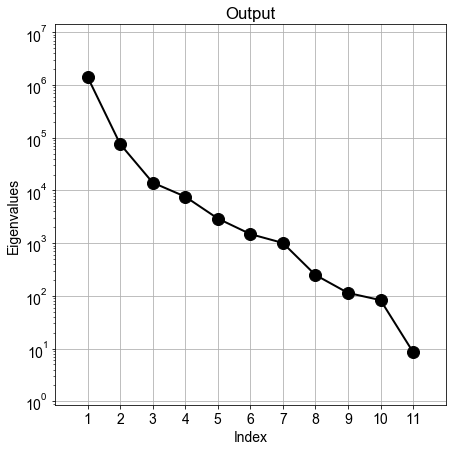
\includegraphics[scale=0.3]{eigs.png} 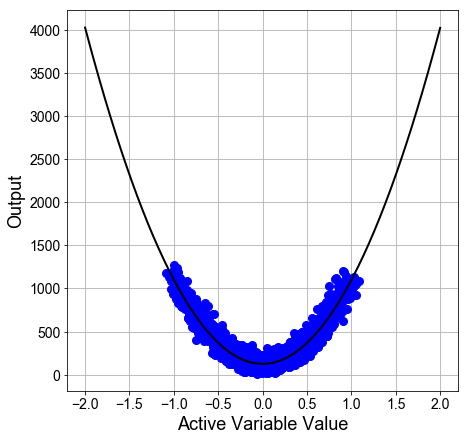
\includegraphics[scale=0.3]{surr.png}

Left: A plot of the eigenvalues of the matrix $\hat{W}$ formed from 1000 Monte Carlo samples in $\Lambda$. We see one dominant eigenvalue on the order of $10^6$. Right: A sufficient summary plot where all 1000 samples are projected into $\A$ and plotted against their function values; a quadratic surrogate fits the projected data with $R^2\approx 0.9$.

\end{center}



\end{frame}

\begin{frame}

\begin{center}

 
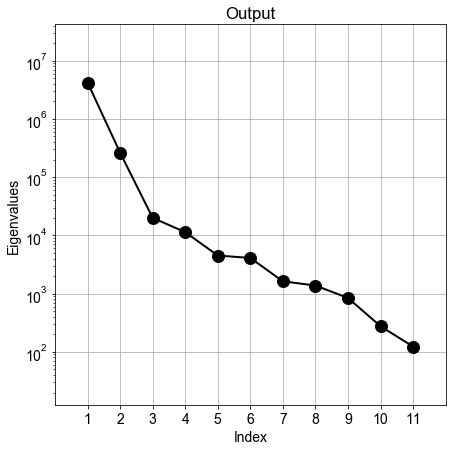
\includegraphics[scale=0.3]{DFO_eigs.png} 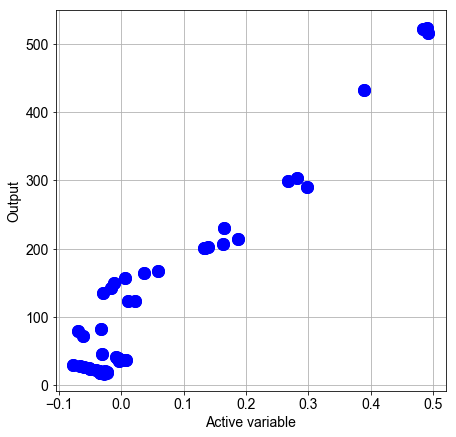
\includegraphics[scale=0.3]{DFO_suffsum.png}

Left: A plot of the eigenvalues of the matrix $\hat{W}$ formed from using 100 DFO iterates as samples in $\Lambda$. We again see one dominant eigenvalue between orders $10^6$ and $10^7$. Right: A sufficient summary plot where all 100 samples are projected into $\A$ and plotted against their function values.

\end{center}



\end{frame}

% ------------------------------------------------
\subsection{Using the Active Subspace}
% ------------------------------------------------

%\begin{frame}

%\begin{itemize}

%	\item Here we consider the effectiveness of DFO performed on $f$ from Example 3 using 500 iterations of unmodified STARS versus a scheme that blends STARS and active subspace analysis using only 150 iterations.
	

%\end{itemize}

%\end{frame}

\begin{frame}


\begin{center}

 
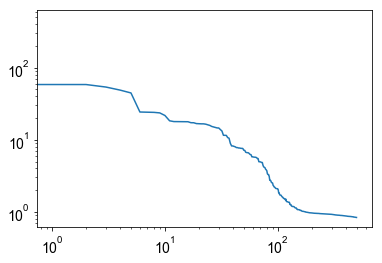
\includegraphics[scale=0.4]{stars.png} 

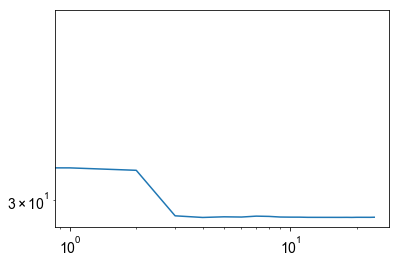
\includegraphics[scale=0.3]{minvec2.png} 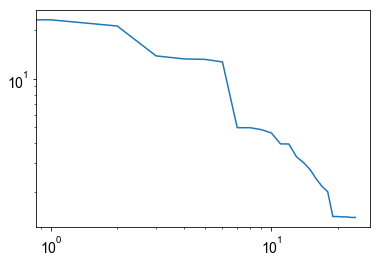
\includegraphics[scale=0.3]{minvec4.png}

Top: 500 iterations of standard DFO; Bottom Left: 25 iterations of minimizing $f$ with DFO along the $\lambda_8$ axis; Bottom Right: 25 iterations of minimizing $f$ with DFO along the $\lambda_6$ axis.

\end{center}


\end{frame}



% ------------------------------------------------
\subsection{Software Dissemination}
% ------------------------------------------------


\begin{frame}

\begin{itemize}

	\item Currently, only some of the software used to produce results in this paper are publicly available on GitHub.com. 
	
	\item Some of the algorithms used here and other algorithms that are of interest are within open-source packages available online \footnotemark[1] \footnotemark[2]. 
	
	\item Special thanks to Michael Pilosov for bringing Active Subspace package into Python 3
	
	\item Other schemes considered here make modifications to given algorithms and remain under development. 
	
	\item A major goal of this thesis proposal will be producing well-documented, open-source software complete with python Jupyter Notebooks containing illustrative, replicable examples.


\end{itemize}

\footnotetext[1]{T. Butler et al}
\footnotetext[2]{Constantine et al}

\end{frame}






% ------------------------------------------------

\section{References}
% ------------------------------------------------
\begin{frame}[allowframebreaks]

%%%%%%%%%%%%%% References %%%%%%%%%%%%%%%%%%%%%%%%%
\begin{thebibliography}{65}

\tiny

\bibitem{battaglia} Battaglia, D. J.  and Burrell, K. H.  and Chang, C. S.  and Ku, S.  and deGrassie, J. S.  and Grierson, B. A. ``Kinetic neoclassical transport in the H-mode pedestal." Physics of Plasmas,Volume 21, No. 7. 2014.


\bibitem{BJW18a} T. Butler and J. Jakeman and T. Wildey.
``Combining Push-Forward Measures and Bayes' Rule to Construct Consistent Solutions to Stochastic Inverse Problems." SIAM Journal on Scientific Computing, Volume 40, No. 2, pp. A984-A1011, 2018.

\bibitem{Calliess} Jan-Peter Calliess. ``Lipschitz optimisation for Lipschitz interpolation." In 2017 American Control Conference (ACC 2017), Seattle, WA, USA, May 2017.

\bibitem{CW} Chen and Wild. ``Randomized Derivative-Free Optimization of Noisy Convex Functions." Funded by the Department of Energy. 2015.

\bibitem{Constantine2015} Constantine, Paul G. ``Active Subspaces: Emerging Ideas for Dimension Reduction in Parameter Studies." SIAM, 2015.

\bibitem{ConstantineMC} Constantine, Eftekhari, Wakin. ``Computing Active Subspaces Efficiently with Gradient Sketching." Conference paper, 2015 IEEE 6th International Workshop on Computational Advances in Multi-Sensor Adaptive Processing (CAMSAP).


\bibitem{KS} Kvasov and Sergeyev. ``Lipschitz gradients for global optimization in a one-point-based partitioning scheme." Journal of Computational and Applied Mathematics. Volume 236, Issue 16, pp. 4042-4054. 2012.

\bibitem{KU_TOTALF} S. Ku and R. Hager and C.S. Chang and J.M. Kwon and S.E. Parker. ``A new hybrid-Lagrangian numerical scheme for gyrokinetic simulation of tokamak edge plasma." Journal of Computational Physics, Volume 315, pp. 467-475. 2016.

\bibitem{Lao85} Lao, L.L, St. John, H, R.D. Stambaugh, A.G. Kellman, and Pfeiffer, W.,``Reconstruction of current profile parameters and plasma shapes in tokamaks'', Nuclear Fusion, Volume 25,No. 11,pp. 1611,1985.

\bibitem{lea2000} Lea, Daniel J. and Allen, Myles R. and Haine, Thomas W. N. ``Sensitivity analysis of the climate of a chaotic system." Tellus A, Volume 52, No. 5, pp. 523-532. 2000.



\bibitem{Russi} Russi, Trent M. ``Uncertainty Quantification with Experimental Data and Complex System Models." Dissertation, University of California Berkeley. 2010.

\bibitem{Smith}  Smith, Ralph.``Uncertainty Quantification: Theory, Implementation, and Applications.” SIAM, 2013.

\bibitem{Stuart} Stuart, Andrew. ``Inverse problems: A Bayesian perspective." Acta Numerica, volume 19, pp. 451-559. 2010.



\bibitem{Tarantola} Tarantola, Albert. ``Inverse Problem Theory and Methods for Model Parameter Estimation." SIAM. 2005.

\bibitem{Takeda91} Takeda, T. and Tokuda S.,``Computation of MHD equilibrium of tokamak plasma'',
Journal of Computational Physics,93,1,1 - 107,1991.

\bibitem{Qiqi2014} Qiqi Wang and Rui Hu and Patrick Blonigan. ``Least Squares Shadowing sensitivity analysis of chaotic limit cycle oscillations." Journal of Computational Physics, Volume 267, pp. 210-224. 2014.


\bibitem{Wesson} Wesson, J. ``Tokamaks." ``Oxford University Press, 4th edition." 2011.

\bibitem{wildeyprez} Wildey, T., Butler, T., Jakeman, J., Walsh, S. " A Consistent Bayesian Approach for Stochastic Inverse Problems Based on Push-forward Measures." SAND2017-3436PE. 2017.


\end{thebibliography}






\end{frame}







\end{document}

